\problemname{One Copenhell of a Problem}

\illustration{.33}{img/crowdsurfer.png}{A panicked student using the crowd to hastily make their way to an exam. Generated using Midjourney.}

This year, the annual metal festival Copenhell will be closed by the band \textit{Algorithmic Power Symphony} that consists solely of students from the nearby IT University. The concert is a huge success, which has resulted in a big problem for all the band members!

The plan was for all of them to attend their final exam in the course "Heavy Metalgorithmic Problem Solving" after ending their concert, but due to the huge demand for encores, they are now running late. The only way for them to reach their exam in time is for them to take advantage of the crowd in front of them and crowdsurf all the way from the stage and to the back of the crowd. Since it is the end of a long festival, all the crowd-members have pretty tired arms from lifting beers and throwing devil-horns, meaning that they can only help lift at most one band member.

How many band members will miss their exam due to not being able to crowdsurf safely all the way to the back of the crowd?

All crowd members in the front row closest to the stage are able to receive a band member and all crowd members in the absolute back row are able to put the band members down so they can start sprinting towards the university.
Once a crowd member receives a band member, they can pass the band member to any of their 8 adjacent crowd members (that is, both orthogonally and diagonally adjacent).

\section*{Input}

The first line of the input consists of three integers $r$, denoting the number of rows in the crowd, $c$, denoting the number of columns in the crowd, and $b$, denoting how many band members are on stage.

Then follow $r$ lines, each containing $c$ characters, describing the crowd. Each character either denotes that a crowd member being present in that cell (\texttt{\#}) or that nobody is there to carry (\texttt{.}). The first row shows the people closest to the scene, and the last row shows the people furthest from the scene.

\section*{Output}

The number of band members not able to crowdsurf all the way from the stage to the back of the crowd. I.e. how many band members will remain standing on the stage.

\section*{Example}

Below, one valid solution for the sample input is illustrated, showing how two band members may be crowdsurfed to the back.

\begin{center}
  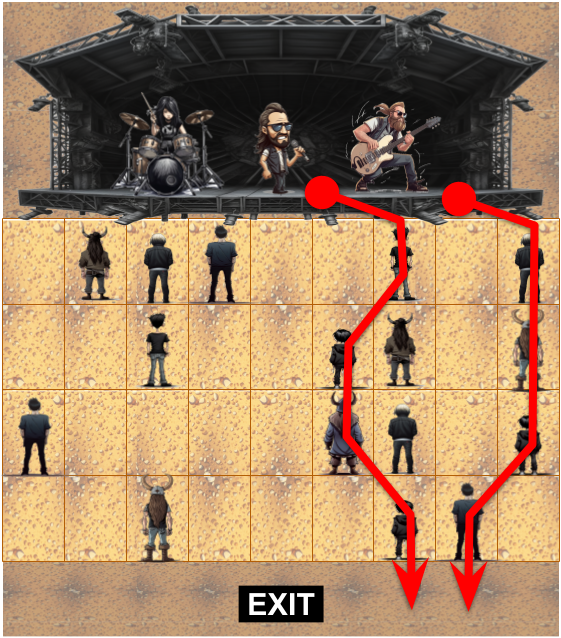
\includegraphics[width=0.4\textwidth]{img/example.png}
\end{center}

The expected output for the example input is 1, because two band members can surf the two rightmost paths, but there is no path from the front to the back via non-exhausted crowd members to carry the third band member, so they will have to remain on stage.

\section*{Scoring}

TBA:..
Sample tests TBA...
